\documentclass[openany,12pt]{book}%openany toglie la pagine bianche tra i capitoli

% Language setting
% Replace `english' with e.g. `spanish' to change the document language
\usepackage[italian]{babel}
\newcommand{\E}{È \hspace{0.1mm}}
\usepackage{import}
% Set page size and margins
% Replace `letterpaper' with `a4paper' for UK/EU standard size
\usepackage[letterpaper,top=2cm,bottom=2cm,left=3cm,right=3cm,marginparwidth=1.75cm]{geometry}

\usepackage{amssymb} % for harpoons
\newcommand{\electron}[2]{{%
        \newcommand*\up{\fbox{$\mathord\upharpoonleft\phantom{\downharpoonright}$}}%
        \newcommand*\dwn{\fbox{$\mathord\downharpoonleft\phantom{\upharpoonright}$}}%
        \newcommand*\updwn{\fbox{$\upharpoonleft\downharpoonright$}}%
        \newcommand*\emp{\fbox{$\phantom{\downharpoonright}\phantom{\downharpoonright}$}}%
        \setlength\tabcolsep{0pt}% remove extra horizontal space from tabular
        \begin{tabular}{c}#2\\[2pt]#1\end{tabular}%
}}
% Useful packages
\usepackage[utf8]{inputenc}
\usepackage{afterpage}
\newcommand\blankpage{%
    \null
    \thispagestyle{empty}%
    \newpage}
\usepackage{amsmath}
\usepackage{graphicx}
\usepackage{hyperref}
\usepackage{array}% only needed for injecting commands at the beginning of columns in the tabular below
\usepackage{electrons}
\usepackage[version=4]{mhchem}
\newcommand{\comment}[1]{}
\usepackage{float}
\usepackage{mathtools}
\usepackage{tikz}
\usetikzlibrary {shapes.geometric}
\usetikzlibrary{decorations.markings}
\usepackage{lipsum}
\usepackage{chemfig}
\usepackage{amsmath}
\usepackage{array}
\setlength\parindent{0pt}%e si gode, toglie lo spostmento a destra di una nuova riga
\usepackage{caption}
\usepackage{subfig}
\usepackage{wrapfig}
\usepackage{float}
\pgfdeclaredecoration{ddbond}{initial}{
  \state{initial}[width=4pt]{
    \pgfpathlineto{\pgfpoint{4pt}{0pt}}
    \pgfpathmoveto{\pgfpoint{2pt}{2pt}}
    \pgfpathlineto{\pgfpoint{4pt}{2pt}}
    \pgfpathmoveto{\pgfpoint{4pt}{0pt}}
  }
  \state{final}{
    \pgfpathlineto{\pgfpointdecoratedpathlast}
  }
}
\tikzset{lddbond/.style={decorate, decoration=ddbond}}
\tikzset{rddbond/.style={decorate, decoration={ddbond, mirror}}}

% #ilchinonlaavràvintaesonoioadecideredovecazzodevestare
\DeclareRobustCommand{\rchi}{{\mathpalette\irchi\relax}}
\newcommand{\irchi}[2]{\raisebox{\depth}{$#1\chi$}} % inner command, used by \rchi

\makeatletter
\newcommand\mathcircled[1]{%
  \mathpalette\@mathcircled{#1}%
}
\newcommand\@mathcircled[2]{%
  \tikz[baseline=(math.base)] \node[draw,ellipse,inner sep=1pt] (math) {$\m@th#1#2$};%
}
\makeatother

\begin{document}

\thispagestyle{empty}
\begin{center}

\begin{minipage}[c]{0.45\textwidth}
\begin{flushleft}

\includegraphics[width=0.8\textwidth]{logo-unict-orizzontale-grigio.png}
\end{flushleft}
\end{minipage}
\hfill
\begin{minipage}[c]{0.45\textwidth}
\begin{flushright}

\includegraphics[width=\textwidth]{logo_dfa_orizzontale}
\end{flushright}
\end{minipage}\\
\medskip
\hbox to \textwidth{\hrulefill}

\vfill
\vfill

\sc{ \Large{Robe a caso poi vediamo}}\vfill
\uppercase{\sc{ \Large{\textbf{Chimica Nino}}}}\\

\vfill
\large{A cura di V. Favitta \& S. Arena }

\vfill
\vfill
\hbox to \textwidth{\hrulefill}
{\sc anno 2022}
\end{center}

\afterpage{\blankpage}

\tableofcontents
\comment{
\chapter{Composizione materia e reazioni chimiche}

\section{Prime nozioni base}%roba a cazzo
\import{./Chapter/1-Sections/}{1-primo}

\section{Nomenclatura}
\import{./Chapter/1-Sections/}{2-secondo}

\section{Differenza tra acido e base}
\import{./Chapter/1-Sections/}{3-terzo}

\section{Base (o dovrei dire idrossido perché si)}
\import{./Chapter/1-Sections/}{4-quarto}

\section{Ossido acido (o dovrei dire anidride)}
\import{./Chapter/1-Sections/}{5-quinto}

\section{Idracidi (no ossigeno)}
\import{./Chapter/1-Sections/}{6-sesta}

\section{Reazioni di salificazione}
\import{./Chapter/1-Sections/}{7-settima}

\section{Reazioni varie}
\import{./Chapter/1-Sections/}{8-ottava}

\section{Ossidoriduzioni}
\import{./Chapter/1-Sections/}{9-nona}

\chapter{Teoria atomica}

\section{Idee bizzarre di fisici bizzarri}
\import{./Chapter/2-Sections}{1-primo}

\section{L'equazione di Schrödinger}
\import{./Chapter/2-Sections}{2-secondo}

\section{Proprietà periodiche}
\import{./Chapter/2-Sections}{3-terzo}

\chapter{Il legame chimico}

\section{Il formalismo di Lewis}
\import{./Chapter/3-Sections}{1-primo}

\section{Geometrie molecolari}
\import{./Chapter/3-Sections}{2-secondo}

\section{La teoria V.S.E.P.R.}
\import{./Chapter/3-Sections}{3-terzo}

\section{Modelli di legame}
\import{./Chapter/3-Sections}{4-quarto}

\chapter{Elementi di termodinamica}

\section{Stato gassoso}
\import{./Chapter/4-Sections}{1-primo}

\section{Stato liquido e cambiamenti di stato}
\import{./Chapter/4-Sections}{2-secondo}

\chapter{Soluzioni acquose}

\section{Soluzioni a due componenti: solvente e soluto}
\import{./Chapter/5-Sections}{1-primo}

\section{La concentrazione}
\import{./Chapter/5-Sections}{2-secondo}

\section{Distillazione}
\import{./Chapter/5-Sections}{3-terzo}

\section{Proprietà colligative}
\import{./Chapter/5-Sections}{4-quarto}

\section{Diagramma di stato o fase}
\import{./Chapter/5-Sections}{5-quinto}

\section{Solubilità}
\import{./Chapter/5-Sections}{6-sesto}

\section{Forze intermolecolari}
\import{./Chapter/5-Sections}{7-settimo}

\section{Tensione superficiale}
\import{./Chapter/5-Sections}{8-ottavo}
}% fine commento

\chapter{L'equilibrio chimico}

\section{Equilibrio chimico omogeneo}
\import{./Chapter/6-Sections}{1-primo}

\section{Acidi e basi}
\import{./Chapter/6-Sections}{2-secondo}

\chapter{Elettrochimica}
\comment{
\appendix

\chapter{Tavola periodica}

\begin{figure}[htp]
  \centering
  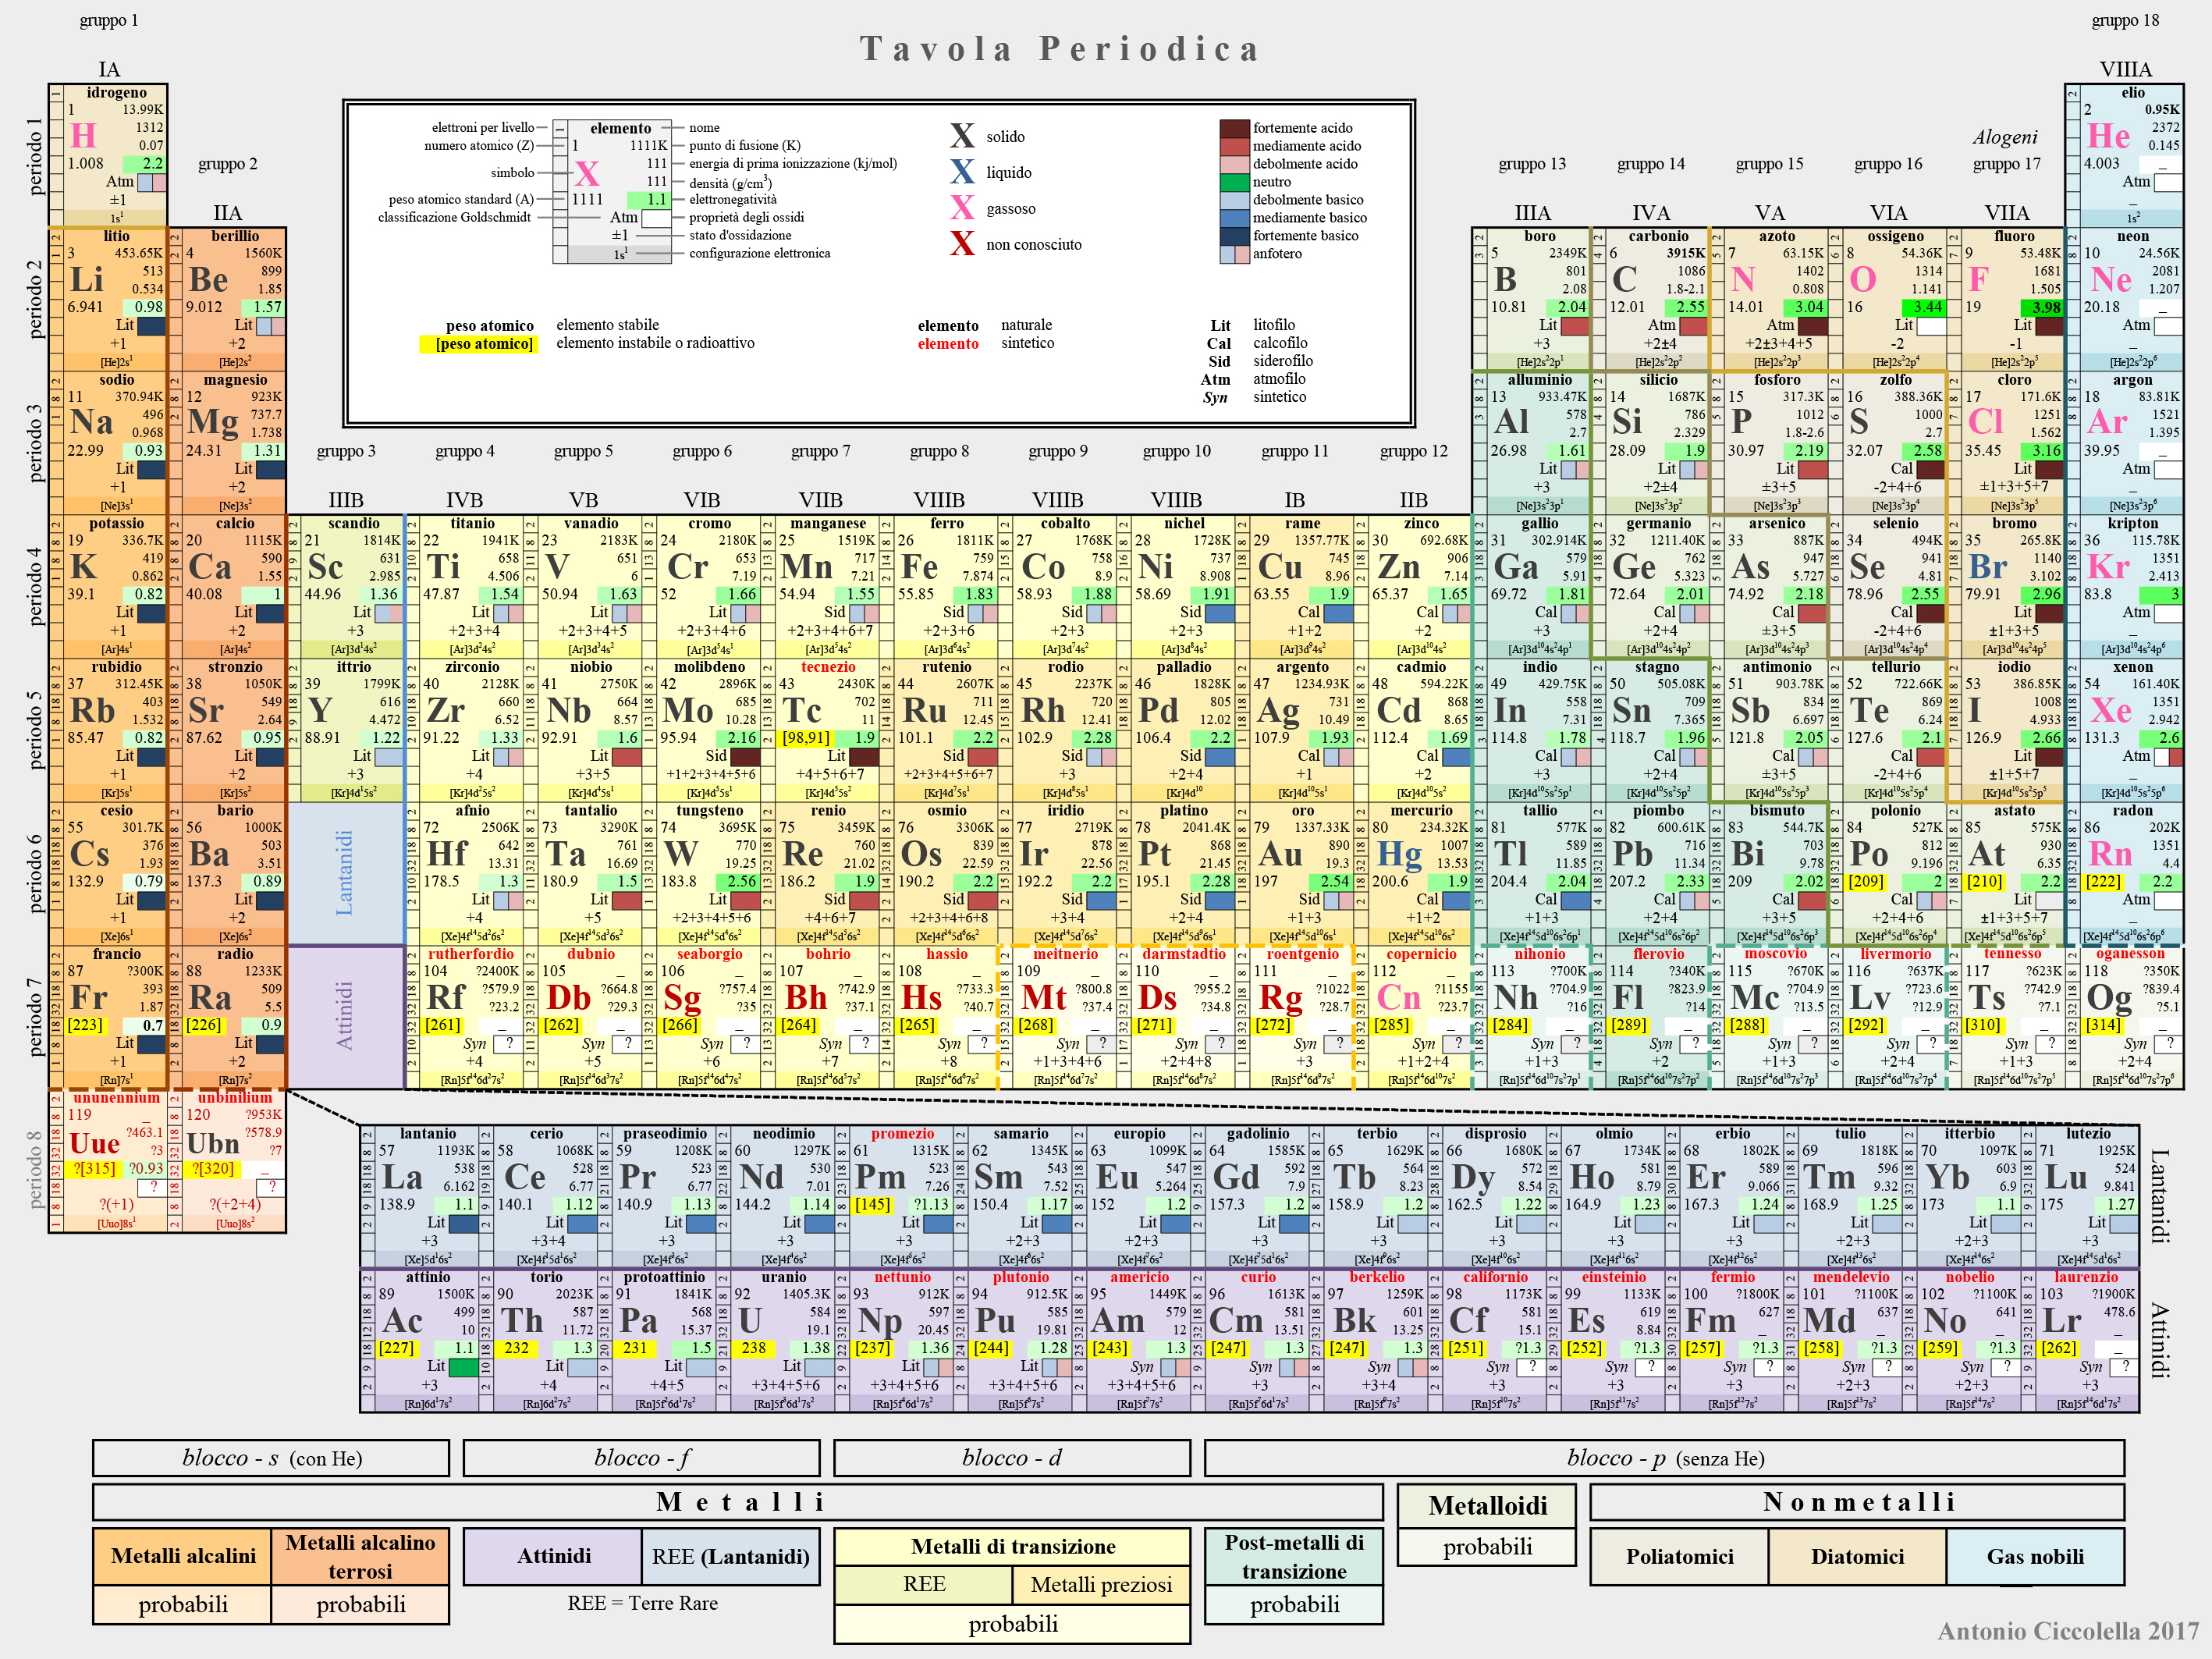
\includegraphics[angle=90,origin=c]{immagini/tavola periodica.png}
\end{figure}
}
\end{document}